\documentclass[UKenglish,usenames,dvipsnames,svgnames,table,aspectratio=169,mathserif]{beamer}

\mode<presentation> {

%\usetheme{default}
\usetheme{Madrid}

\setbeamertemplate{footline} % To remove the footer line in all slides uncomment this line

\setbeamertemplate{navigation symbols}{} % To remove the navigation symbols from the bottom of all slides uncomment this line
}

\usepackage{graphicx} % Allows including images
\usepackage{booktabs} % Allows the use of \toprule, \midrule and \bottomrule in tables
\usepackage{hyperref}
\usepackage{apacite}
\usepackage{babel}
\usepackage{fancyvrb}
\usepackage{color}
\usepackage{alltt}
\usepackage{listings}
\usepackage{framed}
\usepackage{courier}
\usepackage{minted}
\usepackage{epstopdf}
\usepackage{xifthen}
\usepackage[utf8]{inputenc}
\usepackage[T1]{fontenc}
\usepackage{textcomp}
\usepackage{gensymb}
\usepackage{svg}
\usepackage{pdfpages}
\usepackage{isodate}

\hypersetup{colorlinks=false}

\setbeamertemplate{bibliography entry title}{}
\setbeamertemplate{bibliography entry location}{}
\setbeamertemplate{bibliography entry note}{}
\setbeamertemplate{itemize items}[circle]
\setbeamertemplate{enumerate items}[circle]
\beamertemplatenavigationsymbolsempty
\setbeamertemplate{footline}{}


\newminted{haskell}{}
\newminted{scala}{}

\lstdefinelanguage{haskell}{
  morekeywords={class,instance,where,do,data,newtype,default,deriving,module,import,qualified,as},
  otherkeywords={<-},
  sensitive=true,
  morecomment=[l]{--},
  morecomment=[n]{\{-}{-\}},
  morestring=[b]",
  morestring=[b]"""
}

\lstnewenvironment{code}{
  \lstset{
    language=haskell,
    basicstyle=\small\ttfamily,
    stringstyle=\color{olive}\ttfamily,
    escapeinside={*@}{@*},
    showstringspaces=false
  }
}{}

\definecolor{g}{RGB}{0,100,0}
\newcommand{\highlight}[1]{\colorbox{yellow}{#1}}
\newcommand{\nega}[1]{\colorbox{yellow}{#1}}
\newcommand{\posi}[1]{\colorbox{green}{#1}}
\newcommand{\nl}{\vspace{\baselineskip}}
\newcommand{\pnl}{\pause \nl}

\graphicspath{{diagrams/}}

\newcommand{\textslide}[1]{{
\begin{frame}
\begin{center}

#1

\end{center}
\end{frame}
}}

\newcommand{\textslideleft}[1]{{
\begin{frame}

#1

\end{frame}
}}

\newcommand{\codeslide}[1]{{
\begin{frame}[fragile]
\begin{haskellcode}
#1
\end{haskellcode}
\end{frame}
}}

\newcommand{\scalaslide}[1]{{
\begin{frame}[fragile]
\begin{scalacode}
#1
\end{scalacode}
\end{frame}
}}

\newcommand{\imageslide}[2][1]{{
\begin{frame}\begin{center}
\includegraphics[scale=#1]{#2}
\end{center}\end{frame}
}}

\newcommand{\imageslideleft}[2][1]{{
\begin{frame}
\includegraphics[scale=#1]{#2}
\end{frame}
}}

\newcommand{\imagetextslide}[3][1]{{
\begin{frame}\begin{center}

{#3}

\includegraphics[scale=#1]{#2}
\end{center}\end{frame}
}}

\newcommand{\svgslide}[1]{{
\begin{frame}
\begin{center}
\includesvg{diagrams/#1}
\end{center}
\end{frame}
}}

\definecolor{bgc}{RGB}{255, 255, 255}
\setbeamercolor{background canvas}{bg=bgc}


%%----------------------------------------------------------------------------------------
%	TITLE PAGE
%----------------------------------------------------------------------------------------

\title[Contravariant]{Contravariant: The Other Side of the Coin}
\titlegraphic{
\includegraphics[scale=0.2]{data61.eps}}
\author{George Wilson}
\institute[]
{
Data61/CSIRO\\
\medskip
\href{george.wilson@data61.csiro.au}{george.wilson@data61.csiro.au}
}

\selectlanguage{UKenglish}
\date{\printdate{2018-05-22}}

\begin{document}

%%%%%
%%%%% Intro section
%%%%%

\begin{frame}
\titlepage
\end{frame}


\imageslide[0.45]{functor-family-tree.pdf}


% \textslide{\Huge Functor, Applicative, Alternative}


% \begin{frame}[fragile]
% \begin{haskellcode}
% class Functor f where
%   fmap :: (a -> b) -> f a -> f b
% \end{haskellcode}

% \pnl

% \begin{haskellcode}
% class Functor f => Applicative f where
%   (<*>) :: f (a -> b) -> f a -> f b
%   pure  :: a -> f a
% \end{haskellcode}

% \pnl

% \begin{haskellcode}
% class Applicative f => Alternative f where
%   (<|>) :: f a -> f a -> f a
%   empty :: f a
% \end{haskellcode}
% \end{frame}


% \begin{frame}[fragile]
% \begin{haskellcode}
% newtype Parser a = Parser {
%   runParser :: String -> Maybe (a, String)
% }
% instance Functor Parser ...
% instance Applicative Parser ...
% instance Alternative Parser ...
% \end{haskellcode}
% \pnl
% \begin{haskellcode}
% data Json
%   = JObject (Map String Json)
%   | JArray  (Vector Json)
%   | JBool Bool
%   | JString String
%   | JNumber Double
%   | JNull
% \end{haskellcode}
% \end{frame}


% \begin{frame}[fragile]
% \begin{haskellcode}
% jNull :: Parser Json
% jNull = Null <$ string "null"
% \end{haskellcode}

% \pnl

% \begin{haskellcode}
% jKeyValue :: Parser KeyValue
% jKeyValue = KeyValue <$> (jString <* char ':') <*> json
% \end{haskellcode}

% \pnl

% \begin{haskellcode}
% json = :: Parser Json
% json = jObject <|> jArray <|> jNull <|> ...
% \end{haskellcode}
% \end{frame}


\textslide{\Huge Contravariant}


\begin{frame}[fragile]
\begin{haskellcode}
newtype Predicate a =
  Predicate { runPredicate :: a -> Bool}
\end{haskellcode}

\pnl

\begin{haskellcode}
evenP :: Predicate Int
evenP = Predicate (\i -> i `mod` 2 == 0)
\end{haskellcode}

\pnl

\begin{haskellcode}
x :: Bool
x = runPredicate evenP 7
\end{haskellcode}

\end{frame}


\begin{frame}[fragile]
\begin{overlayarea}{\textwidth}{0.2\textheight}
\begin{onlyenv}<1-4>
\begin{haskellcode}
gt5 :: Predicate Int
gt5    = Predicate (\i ->
                      i > 5)
\end{haskellcode}
\end{onlyenv}
\end{overlayarea}

\begin{overlayarea}{\textwidth}{0.25\textheight}
\begin{onlyenv}<2-3>
\begin{haskellcode}
lenGT5 :: Predicate String
lenGT5 = Predicate (\str ->
                      let i = length str
                      in  i > 5)
\end{haskellcode}
\end{onlyenv}
\begin{onlyenv}<4>
\begin{haskellcode}
lenGT5' :: Predicate String
lenGT5' = mapP length gt5
\end{haskellcode}
\end{onlyenv}
\end{overlayarea}

\begin{overlayarea}{\textwidth}{0.25\textheight}
\begin{onlyenv}<3-4>
\begin{haskellcode}
mapP :: (b -> a) -> Predicate a -> Predicate b
mapP ba (Predicate abool) =
  Predicate (\b ->
               let a = ba b
               in  abool a)
\end{haskellcode}
\end{onlyenv}
\end{overlayarea}
\end{frame}


\begin{frame}
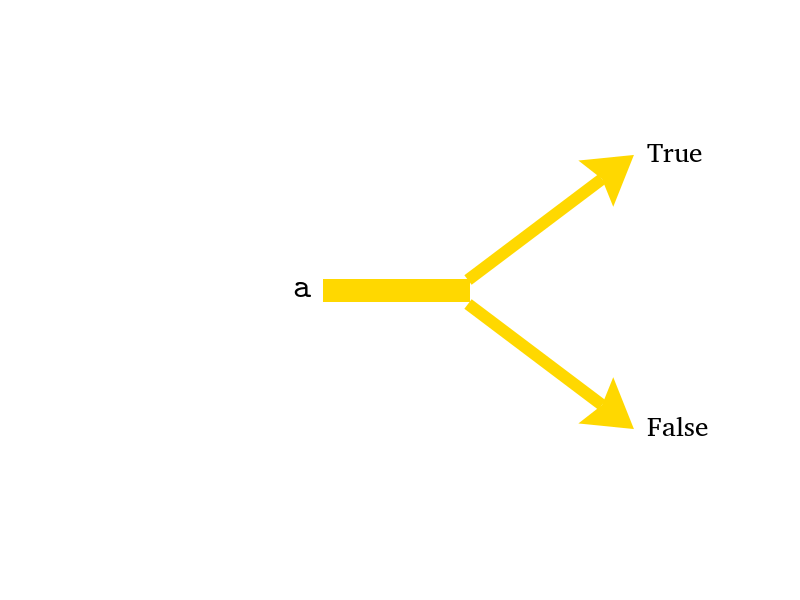
\includegraphics[width=150mm]{pred1.png}
\end{frame}


\begin{frame}
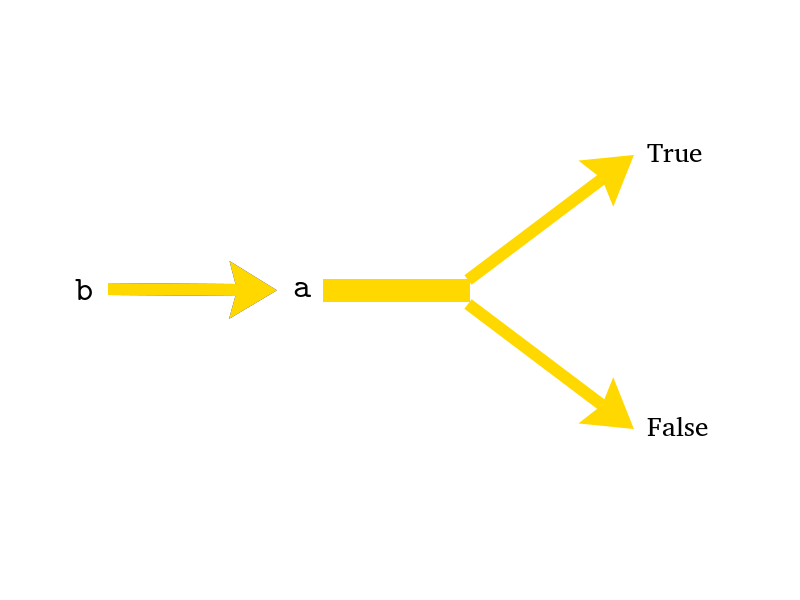
\includegraphics[width=150mm]{pred2.png}
\end{frame}


\begin{frame}[fragile]

Is {\tt Predicate} a {\tt Functor}?

\pnl

\begin{haskellcode}
mapP :: (b -> a) -> Predicate a -> Predicate b
\end{haskellcode}

\begin{haskellcode}
fmap :: (a -> b) -> Predicate a -> Predicate b
\end{haskellcode}

\end{frame}


\begin{frame}
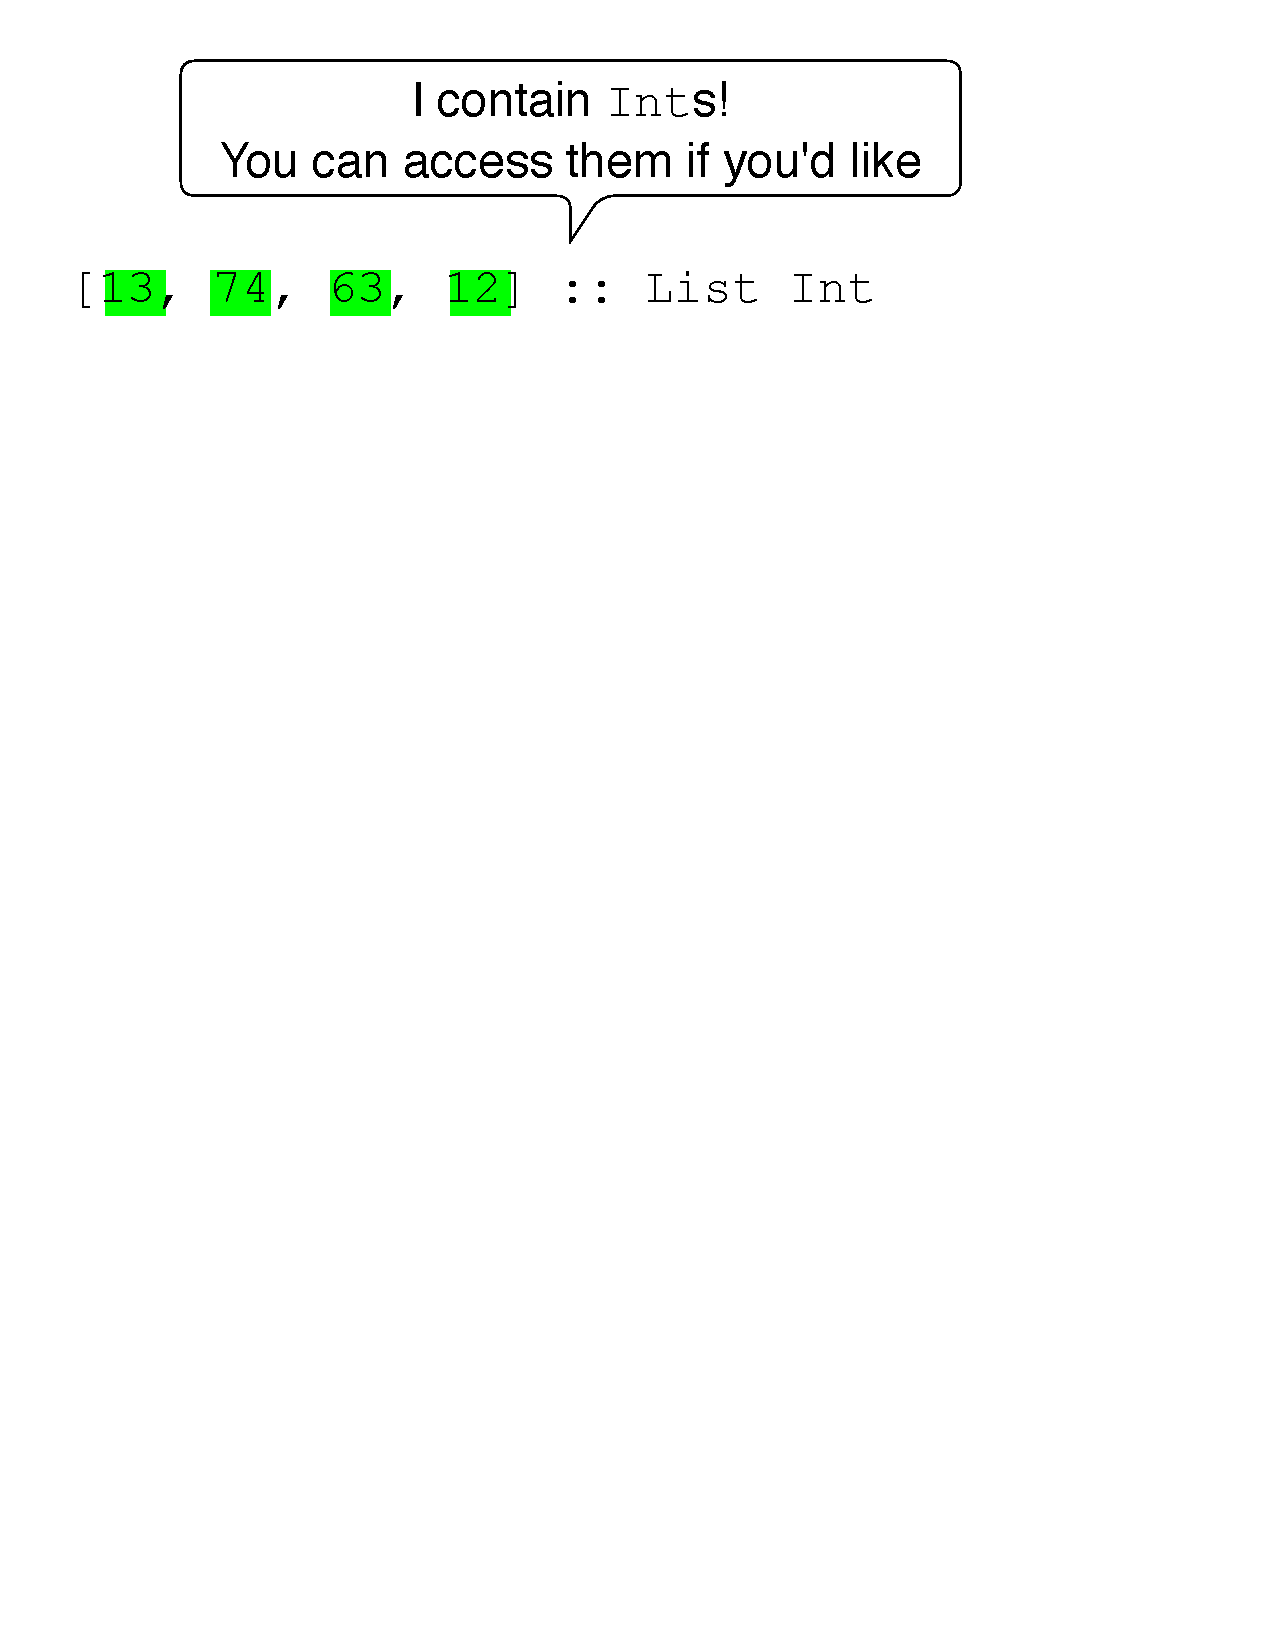
\includegraphics[scale=0.7]{contravariant-want-as1.pdf}
\end{frame}


\begin{frame}
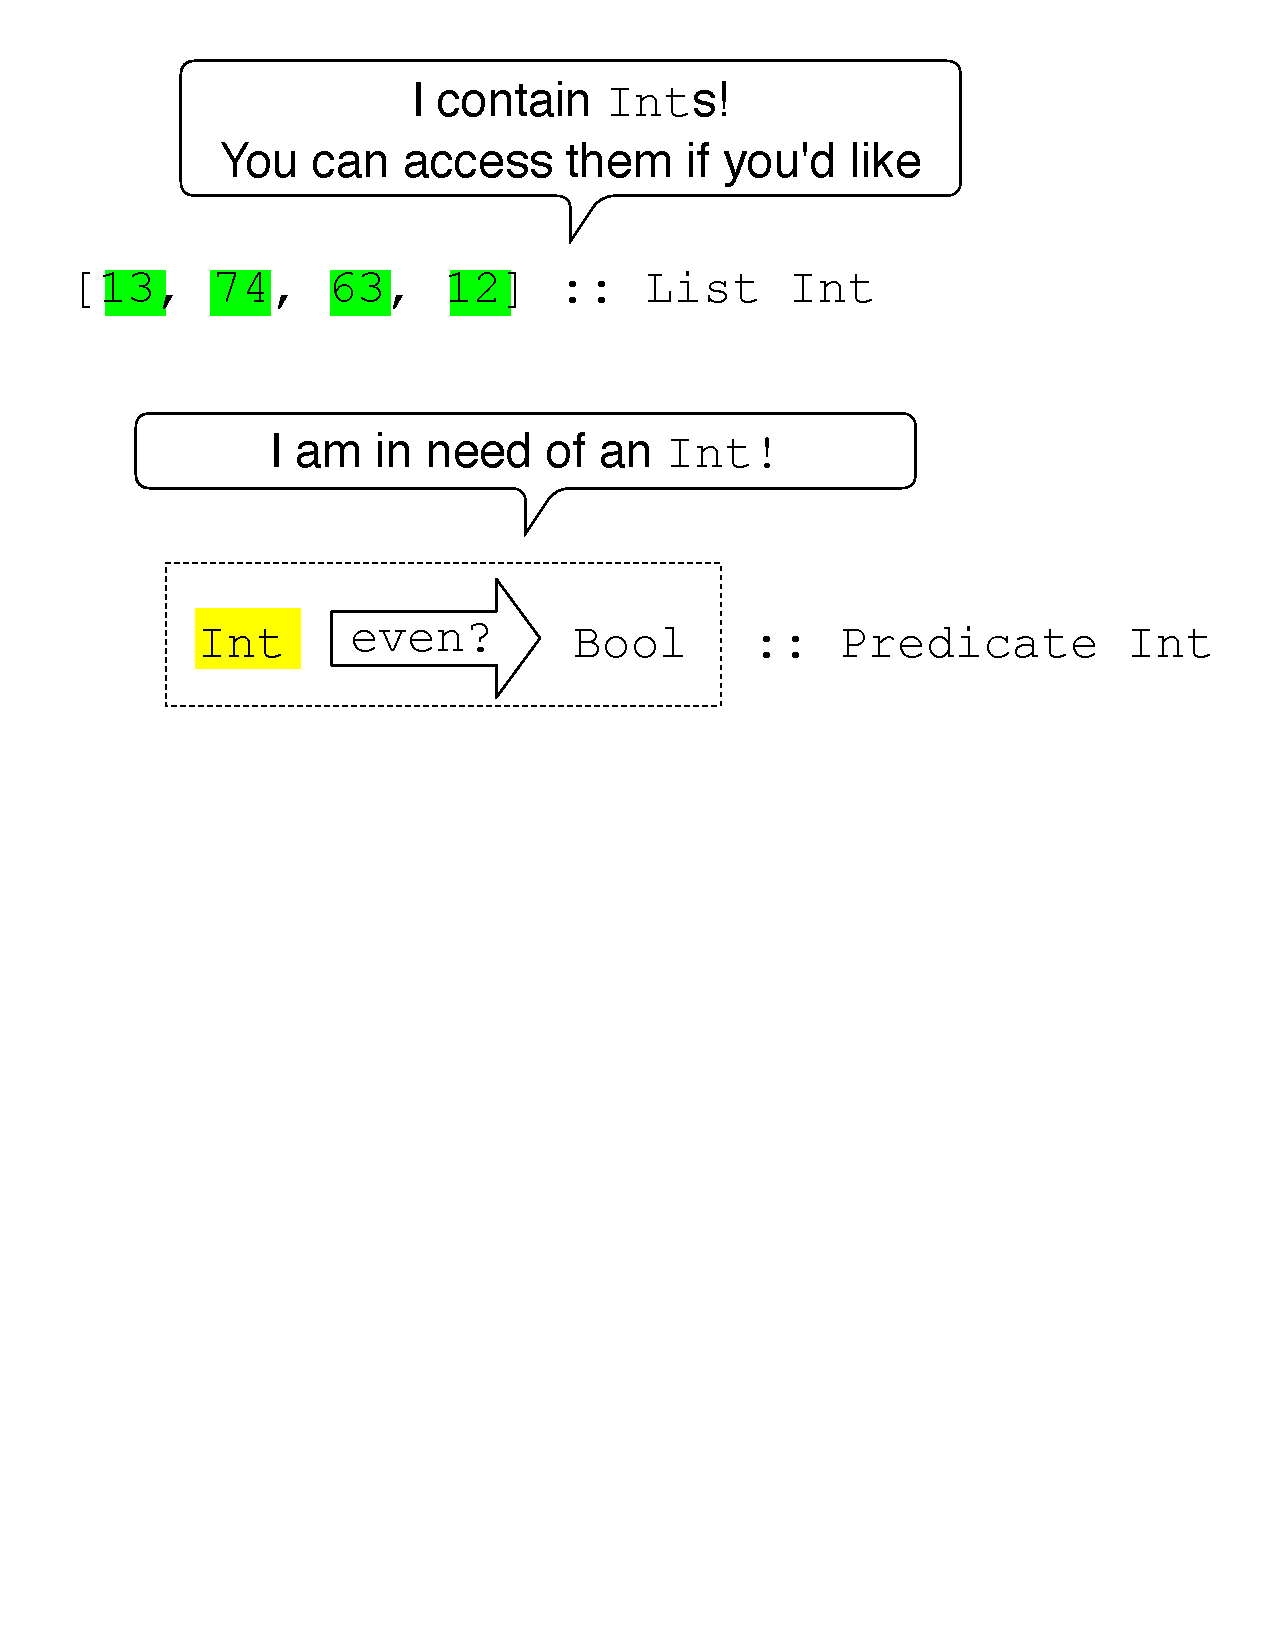
\includegraphics[scale=0.7]{contravariant-want-as2.pdf}
\end{frame}


% \begin{frame}

% A type in a type signature can be in {\it positive} position or in {\it negative} position

% \pnl

% \begin{itemize}
% \item A type on its own is in positive position, like
%   \begin{itemize}
%   \item {\tt i :: \posi{Int}}
%   \item {\tt result :: \posi{Maybe String}}
%   \item {\tt snacks :: \posi{[Banana]}}
%   \end{itemize}
% \pause
% \item Function return types are in positive position, but parameters are in
% negative position
%   \begin{itemize}
%   \item {\tt length :: \nega{[a]} -> \posi{Int}}
%   \item {\tt
%     buildRome :: \nega{Romulus} -> \nega{Remus} -> \posi{Rome}
%   }
%   \end{itemize}
% \end{itemize}

% \end{frame}


% \begin{frame}[fragile]

% If every {\tt a} in {\tt f a} is in positive position

% \nl

% we say that {\tt f} is {\bf covariant} in {\tt a}

% \pnl

% \begin{code}
% data Maybe a = Nothing | Just *@\posi{a}@*
% \end{code}
% \pause
% \begin{code}
% instance Functor Maybe where
%   fmap :: (a -> b) -> Maybe a -> Maybe b
%   fmap f Nothing  = Nothing
%   fmap f (Just x) = Just (f x)
% \end{code}

% \end{frame}


% \begin{frame}[fragile]

% \begin{code}
% newtype Predicate a =
%   Predicate { runPredicate :: *@\nega{a}@* -> Bool }
% \end{code}

% \pnl

% In {\tt Predicate}, we only see {\tt a} in negative position.

% We say {\tt Predicate} is {\bf contravariant} in {\tt a}.

% \end{frame}


\begin{frame}[fragile]
\begin{overlayarea}{\textwidth}{0.5\textheight}

\begin{onlyenv}<1-3>
\begin{haskellcode}
class Contravariant f where
  contramap :: (b -> a) -> f a -> f b
\end{haskellcode}

\nl
\end{onlyenv}

\begin{onlyenv}<2>
Laws:

\begin{itemize}
\item[]
\begin{haskellcode}
contramap id = id
\end{haskellcode}
\item[]
\begin{haskellcode}
contramap f . contramap g = contramap (g . f)
\end{haskellcode}
\end{itemize}
\end{onlyenv}
\begin{onlyenv}<3>
\begin{haskellcode}
instance Contravariant Predicate where
  contramap :: (b -> a) -> Predicate a -> Predicate b
  contramap ba (Predicate abool) = Predicate (abool . ba)
\end{haskellcode}
\end{onlyenv}

\end{overlayarea}
\end{frame}


% \begin{frame}
% \Large
% \begin{center}
% We think of a covariant {\tt Functor} as {\it having} {\tt a}'s.

% A {\tt Contravariant} functor can be thought of as {\it consuming} {\tt a}'s.
% \end{center}
% \end{frame}


\begin{frame}[fragile]
\begin{overlayarea}{\textwidth}{0.2\textheight}
\begin{onlyenv}<1>
\nl
\huge
\begin{center}
We need more power!
\end{center}
\end{onlyenv}
\begin{onlyenv}<2>
\begin{haskellcode}
class Functor f => Applicative  f where
  (<*>)  :: f (a -> b)    -> f a -> f b
  pure   :: a -> f a
\end{haskellcode}
\end{onlyenv}
\begin{onlyenv}<3-4>
\begin{haskellcode}
class Functor f => ApplicativeL f where
  liftA2 :: ((a, b) -> c) -> f a -> f b -> f c
  pure   :: a -> f a
\end{haskellcode}
\end{onlyenv}
\begin{onlyenv}<5-7>
\begin{haskellcode}
class Contravariant f => Divisible f where
  divide  :: (c -> (a, b)) -> f a -> f b -> f c
  conquer :: f a
\end{haskellcode}
\end{onlyenv}
\end{overlayarea}

\nl

\begin{overlayarea}{\textwidth}{0.2\textheight}
\begin{onlyenv}<4>
\begin{haskellcode}
(<*>) :: ApplicativeL f => f (a -> b) -> f a -> f b
(<*>) fab fa = liftA2 (\(ab,a) -> ab a) fab fa
\end{haskellcode}
\end{onlyenv}

\begin{onlyenv}<6>
\small
Laws:

\begin{itemize}
\item[]
\begin{haskellcode}
divide f m conquer = contramap (fst . f) m
\end{haskellcode}
\item[]
\begin{haskellcode}
divide f conquer m = contramap (snd . f) m
\end{haskellcode}
\item[]
\begin{haskellcode}
divide f (divide g m n) o = divide f' m (divide id n o)
  where
    f' a = case f a of (bc,d) -> case g bc of (b,c) -> (a,(b,c))
\end{haskellcode}
\end{itemize}
\end{onlyenv}
\begin{onlyenv}<7>
\begin{haskellcode}
instance Divisible Predicate where
  divide cab (Predicate pa) (Predicate pb) =
    Predicate $ \c ->
      case cab c of
        (a,b) -> pa a && pb b

  conquer = Predicate (\_ -> True)
\end{haskellcode}
\end{onlyenv}
\end{overlayarea}
\end{frame}


\begin{frame}
\centering

\includegraphics[scale=0.09]{images/banana1.jpg}
\end{frame}


\begin{frame}[fragile]

\begin{haskellcode}
ingredients :: (Banana, IceCream)
\end{haskellcode}

\pnl
\begin{haskellcode}
ripe :: Predicate Banana
frozen :: Predicate IceCream
\end{haskellcode}

\pnl
\begin{haskellcode}
divide    :: Divisible f => (c -> (a,b)) -> f a -> f b -> f c
divide id :: Divisible f =>                 f a -> f b -> f (a,b)
\end{haskellcode}

\pnl
\begin{haskellcode}
divide id ripe frozen :: Predicate (Banana, IceCream)
\end{haskellcode}

\pnl
\begin{haskellcode}
runPredicate (divide id ripe frozen) ingredients :: Bool
\end{haskellcode}
\end{frame}


\begin{frame}
\centering
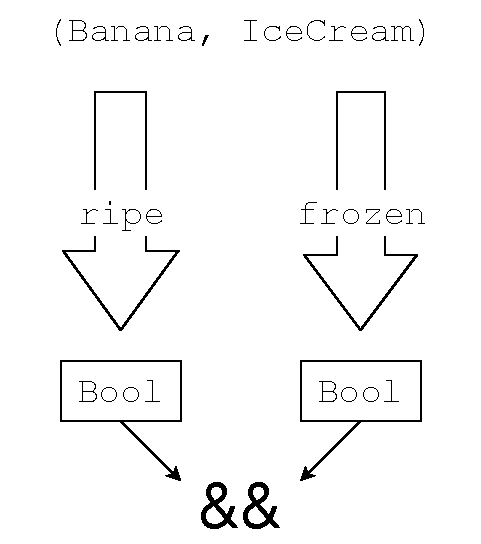
\includegraphics[scale=0.6]{banana1.pdf}
\end{frame}


\begin{frame}[fragile]
\begin{haskellcode}
data Kitchen = Kitchen Rice Curry Banana Apple IceCream
\end{haskellcode}

\pnl
\begin{haskellcode}
ripe :: Predicate Banana
frozen :: Predicate IceCream
\end{haskellcode}

\pnl
\begin{haskellcode}
getIngredients :: Kitchen -> (Banana, IceCream)
getIngredients (Kitchen _ _ b _ i) = (b,i)
\end{haskellcode}

\pnl
\begin{haskellcode}
divide :: Divisible f => (c -> (a,b)) -> f a -> f b -> f c
\end{haskellcode}

\pnl
\begin{haskellcode}
divide getIngredients ripe frozen :: Predicate Kitchen
\end{haskellcode}
\end{frame}


\begin{frame}
\centering
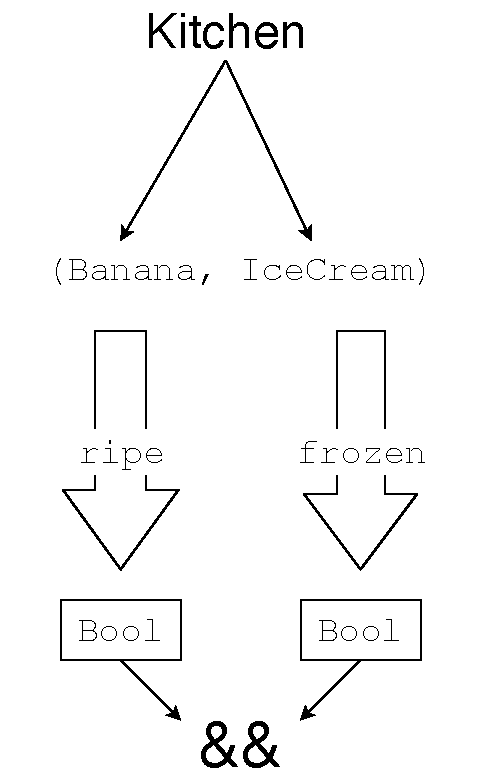
\includegraphics[scale=0.6]{banana2.pdf}
\end{frame}


\begin{frame}
\centering

\includegraphics[scale=0.09]{images/banana2.jpg}
\end{frame}


\begin{frame}
\centering
\huge What about {\tt Alternative}?
\end{frame}


\begin{frame}[fragile]
\begin{haskellcode}
class Contravariant f => Divisible f where
  divide  :: (c -> (a, b)) -> f a -> f b -> f c
  conquer :: f a
\end{haskellcode}
\pnl

\begin{haskellcode}
class Divisible f => Decidable f where
  choose :: (c -> Either a b) -> f a -> f b -> f c
  lose :: (a -> Void) -> f a
\end{haskellcode}

\end{frame}

% \begin{frame}[fragile]
% \begin{overlayarea}{\textwidth}{0.2\textheight}

% % \begin{onlyenv}<1>
% \begin{center}
% \huge
% What about Alternative?
% \end{center}
% \end{onlyenv}
% \begin{onlyenv}<2>
% \begin{haskellcode}
% class Applicative f => Alternative  f where
%   (<|>) :: f a -> f a -> f a
%   empty :: f a
% \end{haskellcode}
% \end{onlyenv}

% \begin{onlyenv}<3>
% \begin{haskellcode}
% class Applicative f => AlternativeE f where
%   (<+>) :: f a -> f b -> f (Either a b)
%   zero  :: f Void
% \end{haskellcode}
% \end{onlyenv}
% \end{overlayarea}

% \end{frame}


\begin{frame}[fragile]
\begin{haskellcode}
data Void

absurd :: Void -> a
absurd v = case v of {}
\end{haskellcode}

\pnl

\begin{haskellcode}
left :: Either a Void -> a
left = either id absurd

right :: Either Void b -> b
right = either absurd id
\end{haskellcode}
\end{frame}


\begin{frame}[fragile]
\begin{overlayarea}{\textwidth}{0.5\textheight}

\begin{haskellcode}
class Divisible f => Decidable f where
  choose :: (c -> Either a b) -> f a -> f b -> f c
  lose :: (a -> Void) -> f a
\end{haskellcode}

\nl

\begin{onlyenv}<2>
\small
Laws:
\begin{itemize}
\item[]
\begin{haskellcode}
choose Left m (lose f)  = m
\end{haskellcode}
\item[]
\begin{haskellcode}
choose Right (lose f) m = m
\end{haskellcode}
\item[]
\begin{haskellcode}
choose f (choose g m n) o = choose f' m (choose id n o) where
  f' bcd = either (either id (Right . Left) . g) (Right . Right) . f
\end{haskellcode}
\end{itemize}
\end{onlyenv}

\begin{onlyenv}<3>
\begin{haskellcode}
instance Decidable Predicate where
  choose cab (Predicate pa) (Predicate pb) =
    Predicate $ \c ->
      case cab c of
        Left a -> pa a
        Right b -> pb b

  lose av = Predicate (\a -> absurd (av a))
\end{haskellcode}
\end{onlyenv}
\end{overlayarea}

\end{frame}


% \begin{frame}[fragile]
% \begin{centering}
% \begin{haskellcode}
%                            data Void
% \end{haskellcode}
% \pause
% \begin{haskellcode}
%                            absurd :: Void -> a
% \end{haskellcode}

% \end{centering}
% \end{frame}


% \begin{frame}[fragile]
% \Large
% \begin{Verbatim}
%                          x

%                        (x,())

%                        ((),x)
% \end{Verbatim}
% \end{frame}


% \begin{frame}[fragile]
% \Large
% \begin{Verbatim}
%                          x

%                     Either x Void

%                     Either Void x
% \end{Verbatim}
% \end{frame}


\begin{frame}
\Huge \centering
Predicates are boring
\end{frame}


% \begin{frame}[fragile]

% {\Large Parsers are exciting! \\}

% \begin{haskellcode}
% jNull :: Parser Json
% jNull = Null <$ string "null"
% \end{haskellcode}

% \nl

% \begin{haskellcode}
% jKeyValue :: Parser KeyValue
% jKeyValue = KeyValue <$> (jString <* char ':') <*> jValue
% \end{haskellcode}

% \nl

% \begin{haskellcode}
% json = :: Parser Json
% json = jObject <|> jArray <|> jNull <|> ...
% \end{haskellcode}
% \end{frame}


\begin{frame}[fragile]
% \begin{haskellcode}
% newtype Parser a = Parser {
%   runParser :: String -> Maybe (a, String)
% }
% \end{haskellcode}

% \pnl

\begin{haskellcode}
newtype Printer a = Printer {
  runPrinter :: a -> String
}
\end{haskellcode}
\end{frame}


\begin{frame}[fragile]
\begin{haskellcode}
string :: Printer String
string = Printer id

konst :: String -> Printer a
konst s = Printer (const s)

showP :: Show a => Printer a
showP = Printer show

int :: Printer Int
int = showP

newline :: Printer ()
newline = konst "\n"
\end{haskellcode}
\end{frame}


\begin{frame}[fragile]
\begin{haskellcode}
instance Contravariant Printer where
  contramap ba (Printer as) = Printer (as . ba)
\end{haskellcode}
\pnl
\begin{haskellcode}
instance Divisible Printer where
  divide cab (Printer as) (Printer bs) = Printer $ \c ->
    case cab c of
      (a,b) -> as a <> bs b

  conquer = Printer (const "")
\end{haskellcode}
\end{frame}


\begin{frame}[fragile]
\begin{haskellcode}
instance Decidable Printer where
  choose cab (Printer as) (Printer bs) = Printer $ \c ->
    case cab c of
      Left  a -> as a
      Right b -> bs b

  lose av = Printer (\a -> absurd (av a))
\end{haskellcode}
\end{frame}


\begin{frame}[fragile]
\begin{haskellcode}
(>$<) :: Contravariant f => (b -> a) -> f a -> f b
(>$<) = contramap
\end{haskellcode}
\pause
\begin{haskellcode}
(>*<) :: Divisible f => f a -> f b -> f (a,b)
(>*<) = divide id
\end{haskellcode}
\pause
\begin{haskellcode}
(>|<) :: Decidable f => f a -> f b -> f (Either a b)
(>|<) = choose id
\end{haskellcode}
\pause
\begin{haskellcode}
(>*) :: Divisible f => f a -> f () -> f a
(>*) = divide (\a -> (a,()))
\end{haskellcode}
\begin{haskellcode}
(*<) :: Divisible f => f () -> f a -> f a
(*<) = divide (\a -> ((),a))
\end{haskellcode}
\end{frame}


\begin{frame}[fragile]
\begin{haskellcode}
infixr 3 >$<

infixr 4 >*<

infixr 3 >|<

infixr 4 >*

infixr 4 *<
\end{haskellcode}
\end{frame}


\begin{frame}[fragile]
\begin{haskellcode}
data Car = Car
  { make   :: String
  , model  :: String
  , engine :: Engine
  }

data Engine = Pistons Int | Rocket
\end{haskellcode}
\pnl
\begin{haskellcode}
car :: Car
car = Car "Toyota" "Corolla" (Pistons 4)
\end{haskellcode}
\end{frame}


\begin{frame}[fragile]
\begin{haskellcode}
engineToEither :: Engine -> Either Int ()
engineToEither e = case e of
  Pistons i -> Left i
  Rocket    -> Right ()

enginePrint :: Printer Engine
enginePrint =
  engineToEither
    >$< konst "Pistons: " *< int
    >|< konst "Rocket"
\end{haskellcode}
\end{frame}

\begin{frame}[fragile]
\begin{haskellcode}
carToTuple :: Car -> (String, (String, Engine))
carToTuple (Car ma mo e) = (ma, (mo, e))

carPrint :: Printer Car
carPrint =
  carToTuple
    >$< (konst "Make:  " *< string >* newline)
    >*< (konst "Model: " *< string >* newline)
    >*< enginePrint
\end{haskellcode}
\end{frame}


\begin{frame}[fragile]
\begin{haskellcode}
putStrLn $ runPrinter carPrint car
\end{haskellcode}

\begin{block}

\begin{code}
Make:  Toyota
Model: Corolla
Pistons: 4
\end{code}
\end{block}
\end{frame}


\begin{frame}

\Large
\begin{itemize}
\item {\tt Applicative} and {\tt Alternative} let us talk about how to \\
      {\it combine} multiple {\it results}
\item {\tt Divisible} and {\tt Decidable} let us talk about how to \\
      {\it consume} multiple {\it inputs}
\end{itemize}

\end{frame}


% \begin{frame}[fragile]
% \frametitle{Discrimination}

% \begin{haskellcode}
% newtype Sort a = Sort { runSort :: forall b. [(a,b)] -> [[b]] }
% \end{haskellcode}
% \pnl
% \begin{haskellcode}
% instance Contravariant Sort where ...
% instance Divisible     Sort where ...
% instance Decidable     Sort where ...
% \end{haskellcode}
% \end{frame}


%\input{contravariant/comparison.tex}


% \begin{frame}[fragile]
% \begin{haskellcode}
% between :: Printer a -> Printer b -> String -> Printer (a,b)
% between a b sep = a >*< (konst sep *< b)

% (>*~<) :: Printer a -> Printer b -> Printer (a,b)
% (>*~<) a b = (a >* konst " ") >*< b 

% (>*|<) :: Printer a -> Printer b -> Printer (a,b)
% (>*|<) a b = (a >* konst "\n") >*< b 
% \end{haskellcode}
% \end{frame}


\begin{frame}
\centering
\Huge
Thanks for listening!

\nl

Questions?
\end{frame}


\begin{frame}
\frametitle{References}

\begin{itemize}
\item \url{https://hackage.haskell.org/package/contravariant}
\item \url{https://github.com/qfpl/invariant-extras}
\item \url{https://hackage.haskell.org/package/generics-eot}
\item Discrimination is Wrong \\
      \url{https://www.youtube.com/watch?v=eXDJ5Jcbgk8}
\end{itemize}

\end{frame}


\begin{frame}[fragile]

{\Large
``Is there a contravariant {\tt Monad}?'' No
}

\nl

\begin{haskellcode}
class Applicative f => MonadJ f where
  join :: f (f a) -> f a
\end{haskellcode}

but

\begin{haskellcode}
newtype Compose f g a = Compose (f (g a))

instance (Contravariant f, Contravariant g) =>
  Functor (Compose f g) where
  fmap z (Compose fga) = Compose $ contramap (contramap z) fga
\end{haskellcode}
\end{frame}


\begin{frame}[fragile]

{\Large
``Is anything both contravariant and covariant?''
}
\nl

\begin{haskellcode}
data Const c a = Const c

instance Functor (Const c) where
  fmap f (Const c) = Const c

instance Contravariant (Const c) where
  contramap f (Const c) = Const c
\end{haskellcode}

\nl

Every {\tt a} is in positive position

Every {\tt a} is in negative position

\end{frame}

\end{document}
